This chapter will analyse how accurate the IPS produced is and will critically analyse the delivered solution. The requirements from chapter 3 will provide the basis for the functional evaluation of the project. Furthermore, the project will be evaluated from a non-functional perspective, as well. The last section will provide a comparison between the existing solutions and the solution developed by our project.
% Each of the functional requirements specified in chapter 4 will be used for this evaluation. Furthermore, the project will be discussed from a non-functional perspective as well. The last section will look into the limitations mentioned in section \ref{sec:limitations}, and how this have affected developing and using the system.

\section{IPS Performance and Accuracy Analysis}
\label{sec:accuracy}

The data was mainly collected from the South Wing of Bush House in this project, mostly due to the fact that the North Wing is the academic area. The data collection has started using only one computer lab, and progressively the data set has been extended from the corridor, to the computer labs around, and to the other floors. It has been assumed that if the algorithm performs well on a small and restricted data set, such as one or two rooms, which are very close to each other, on a larger scale, the performance should stay the same, if not improve. Only one wing of Bush House has been mainly used for testing, because on the other wing, the academic offices are found, and the area is slightly restricted. 

To evaluate the IPS, the data collection has been made using the admin application that has run on an iPad, because the screen is bigger and tapping on certain locations to record is more precise. For the user application that only requests the current position and shows paths to certain destinations, an iPhone has been used. It is strongly recommended that data collection is done on a tablet due to the higher amount of precision.

The positioning algorithm has been tested in different scenarios. First, given a data set, the goal of the tests were to position the user as accurate as possible in a room where the measurements are known. Measurements have been recorded having approximately 2m between themselves. However, certain positions in a room have been inaccessible due to the position of the chairs or tables. Taking this into account, the algorithm places the user in the location that matches the data set the best, therefore, the accuracy of the algorithm is about 1-2 meters. The results given this configuration can be seen in figure 6.1. 

\begin{figure}[H]
    \centering
    \fbox{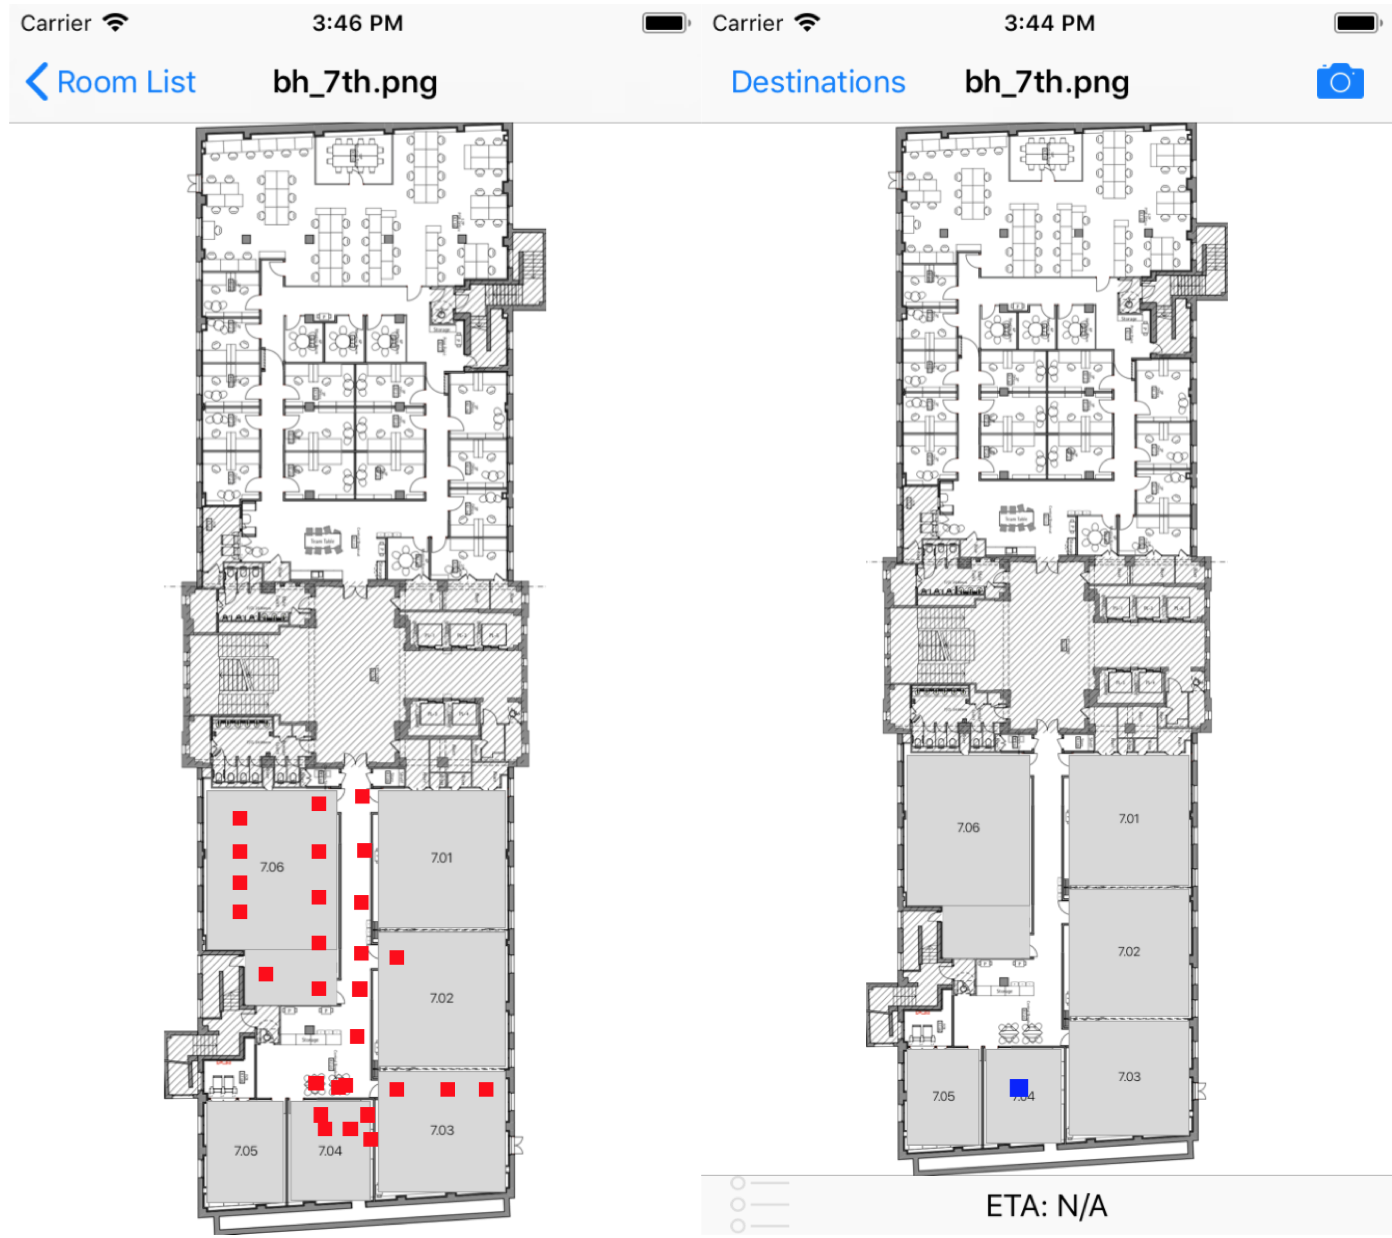
\includegraphics[width=300px, height=268px]{Evaluation/known-loc.png}}
    \caption{Positioning with known locations. The squares in red represent the recorded locations and the square in blue represents the position determined by the algorithm. The screenshot on the left is from the admin application, and the screenshot on the right is from the user application.}
    \label{fig:ips-known-loc}
\end{figure}

\newpage
The second scenario the algorithm has been tested was when data has not been measured for a room, but there are close measurements to the current position. In this case, the algorithm gradually positions the user on the closest recorded position to the current position. The results for this can be observed in figure 6.2.

\begin{figure}[H]
    \centering
    \fbox{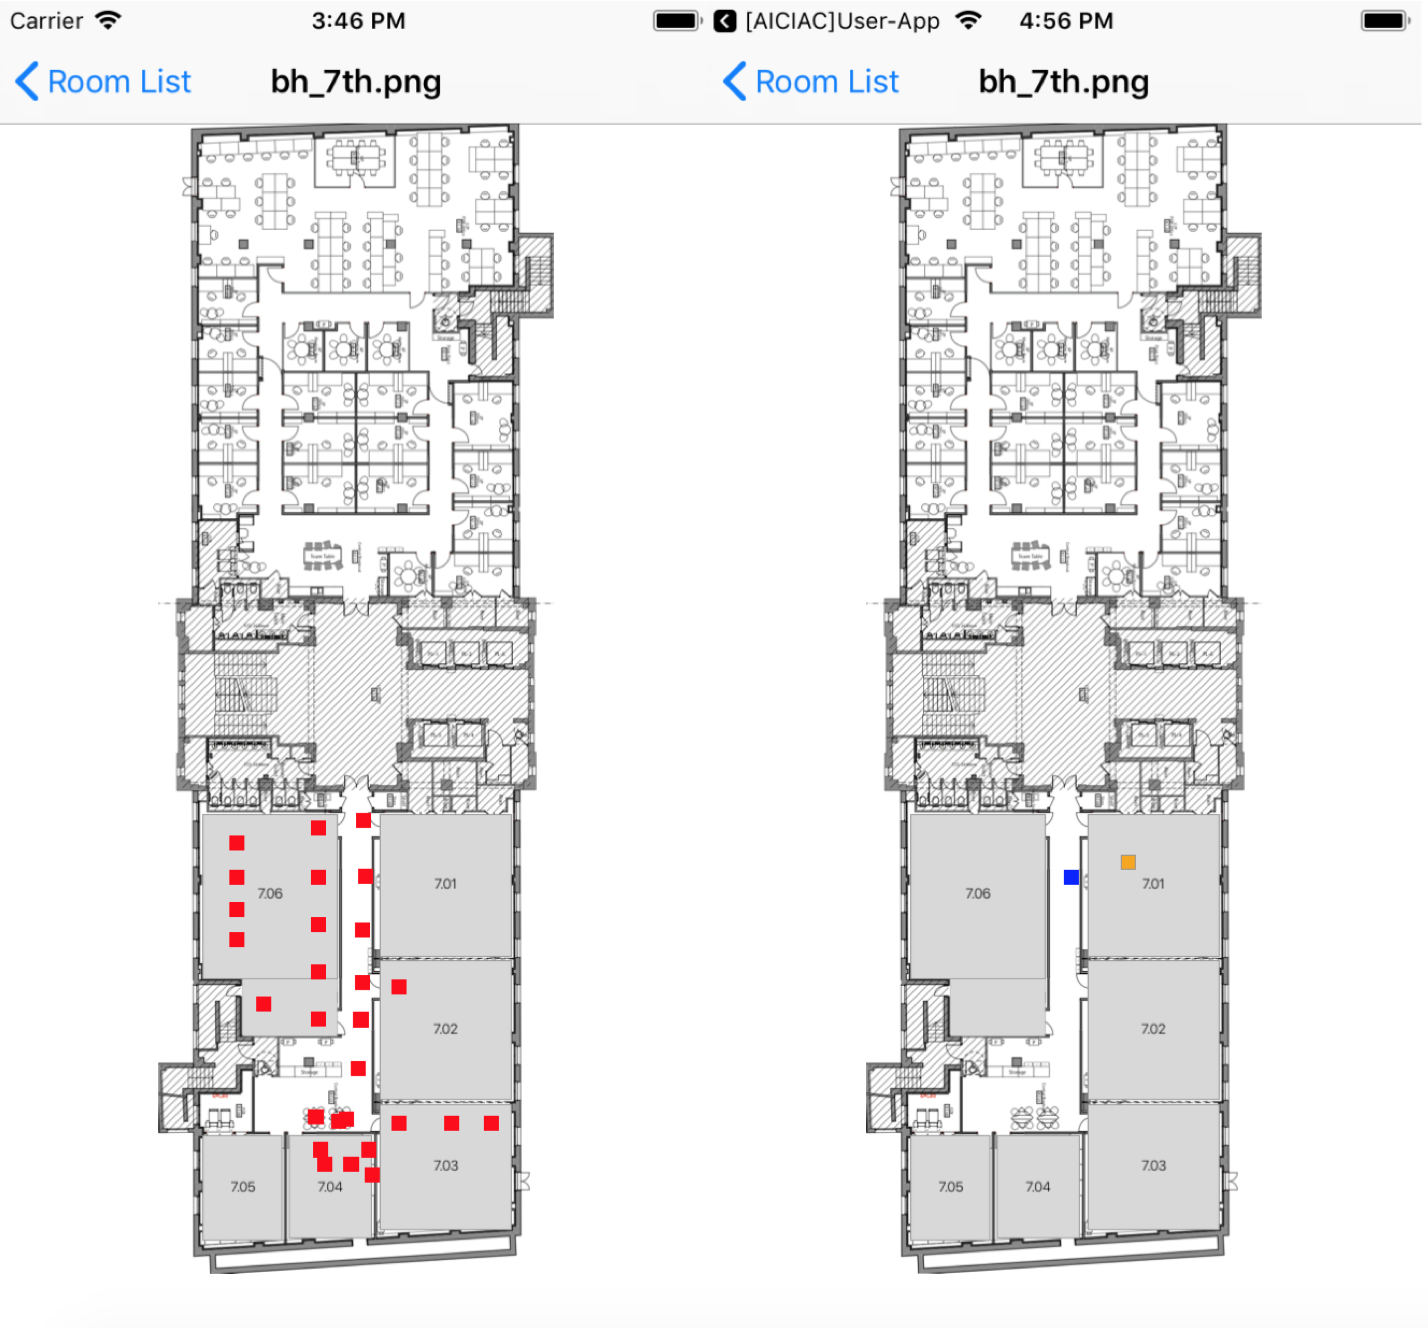
\includegraphics[width=300px, height=279px]{Evaluation/unknown-loc.png}}
    \caption{Positioning with unknown locations in the room where the user is. The squares in red represent the recorded locations. The square in blue represents the position determined by the algorithm, and the square in light orange is the actual position of the user. }
    \label{fig:ips-unknown-loc}
\end{figure}

\section{Navigation Algorithm Analysis}

The testing approach for the navigation algorithm has been the same as the one for the IPS. The algorithm has been tested first with locations in the same room, then between two adjacent rooms, and then from wing to wing. In order to test the algorithm, convenient positions have been recorded in order for the path to be shown in a user friendly way on the floor plan (e.g. in front of doors; in this way the path will line up perfectly on the screen and they will not be placed on top of walls). One of the large scale tests has been from the end of the South Wing to my supervisor's office. It can be seen in figure 6.3 that the algorithm has been successful in finding a path between the two locations.

\begin{figure}[H]
    \centering
    \fbox{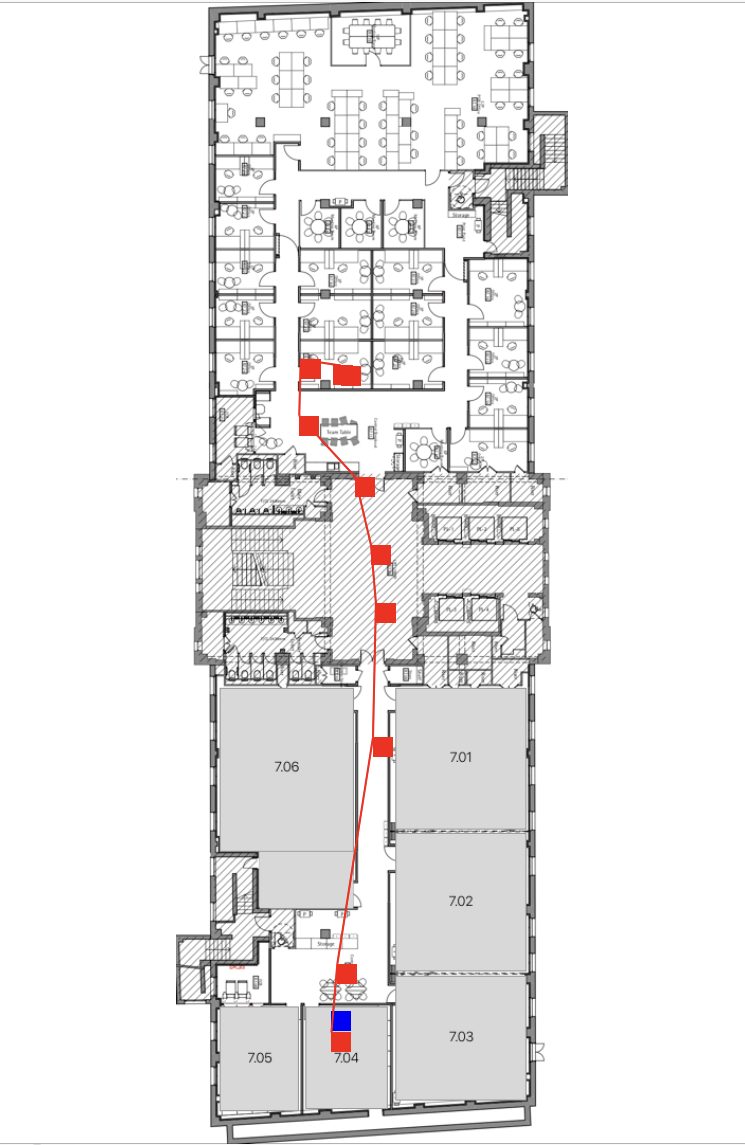
\includegraphics[width=180px, height=280px]{Evaluation/long-path.png}}
    \caption{Long path between a computer lab in the South Wing and an office on the North Wing of Bush House. The square in blue represents the current position of the user and the squares in red represent the way-points to follow. The last red square represents the destination.}
    \label{fig:nav-long-path}
\end{figure}

\section{Project Evaluation}

\subsection{Functional Evaluation}
When taking into consideration the requirements set in chapter 4, it can be said that the project has fully achieved and met all of them. All of them can be fully tested. In fact, the project is able to scan and save Wi-Fi measurements, use them to position a user, and then provide navigation instructions for users to find their way around Bush House. However, it is very difficult to assess some of the requirements, and evaluating some of them is irrelevant to the project aims; requirements like that are "RPS3 – Check continuously if data is needed", or "WSS1 – Have a Boolean flag to know if data needs to scanned or not". An empirical evaluation of the project that looks at how accurate the system is has been provided in section \ref{sec:accuracy}, and a non-functional evaluation, focused more on quality attributes, will be further detailed in the following section.

\subsection{Non-functional Evaluation}
\begin{itemize}
    \item Interoperability – The subsystems should be able to fully integrate with other subsystems in order to provide maximum flexibility.
    
    As mentioned in the design chapter and in the implementation chapter, all the servers and data providers provide an API to communicate with other components of the system. The data management server has a RESTful API to access the database, the Positioning \& Path Finder system has an API in order to calculate data and provide results, and the AR Data Provider has an API that provides required data to show in the user application. All the communications that take place using the APIs use a JSON format, which is a very popular serialisation format.
    
    \item Maintainability – The system should be provide a simple and easy way to extend feature base. For this, the follow concepts must be followed:
        \begin{itemize}
            \item Separation of Systems – The system must be decomposed in multiple independent subsystems which must be as decoupled as possible. The systems should use the appropriate programming languages and framework to achieve their requirements and tasks.
            \newline\newline
            The architecture components have been separated first into layers that achieve common goals, and then into separate systems, depending on the task achieved. The user mobile application and admin mobile application have been separated due to the nature of the features, and then based on the data that each handles, the other systems have been decoupled. This is detailed extensively in the design chapter. Because systems are very separated, any of them can be easily replaced without affecting the system as a whole. For example, mobile applications could be developed for other operating systems, such as Android.
            \item Architectural Patterns – Each subsystem should follow the appropriate architectural pattern and design patterns provided by the framework that is being used, or the programming language that the system is written in.
            \newline\newline
            The best practices and design patterns have been used when appropriate, in each application. Most of the system makes use of an MVC design pattern, mainly due to the frameworks that they use, and the way those have been designed. Evidence stands from the details presented in the design chapter, along with the code listed in the implementation chapter and the appendix.
        \end{itemize}
    \item Usability – The system should provide an easy to use interface, and as clear as possible. Although it can be simple, the interfaces must provide clarity of interactions, and a satisfactory user experience.
    \newline\newline
    The graphical user interface of the mobile applications has been made very clear and very simple. Moreover, during the design and development phases, the user feedback that has been received regarding this has been used whenever possible, in other for the GUI to be very clear to use.
\end{itemize}

% \subsection{Limitations}

% In results, talk about the overhead that the HTTP request bring for example to the positioning algorithm, or even the navigation algorithm.

\section{Comparison to other existing solutions}
When it comes to compare the functionalities and capabilities, along with the way of working of the application built, the most suitable comparison would be with "Indoor Survey App" \cite{apple-indoor-survey}. The comparison with the application built by Apple is the most relevant, since the way of measuring data for location is very similar, but our solution provides an arguably better and more extensible system.

The most important comparison that can be made with Apple's solution is the architecture of the system. A very important aspect to remember is that Indoor Survey App provides positioning and measuring for any building that follows their specific requirements, whereas our solution only supports Bush House. However, this is a feature that can be easily added on top of the existing capabilities, since our system has been developed with extensibility in mind.

The way that both of the application measure relevant positions in the buildings is by using the floor plans. After the user registers their floor plans and has them available in the application, they can record important reference points in the building by tapping on the screen. This will register that position on the image and assign Wi-Fi measurements to it. Even though the way of working is more or less the same, our system can support any measuring platform, let it be for example Android, whereas Apple's will only run on iOS. However, performance-wise, Apple's application is faster when dealing with scanning for Wi-Fi networks, because all the measurements take place on the phone, and not through a multitude of systems, as ours does. Nevertheless, if the scanning functionality would be open to anyone, this can be easily adopted by our application without any difficulties. This will be detailed in the conclusion chapter.

Furthermore, Apple's application is limited to buildings and venues that "attract more than one million visitors annually" \cite{apple-indoor-survey}. Although our system only supports Bush House, as previously mentioned, as future work, it can be easily extended to any building that has its floor plans available. It is not clear right now if Apple's application supports anything more than just measuring buildings and then positioning users, but our system comes at an advantage because our solution brings navigation and also makes use of AR features by using ARKit to improve the user's experience.

Another solution that has a fingerprinting based approach is SLAM \cite{SLAM}. SLAM tries to improve this approach by eliminating the offline measuring process, which brings a lot of limitations by the fact that the area must be surveyed before using the positioning system. This solution brings tracking on unknown grounds and requires no prior knowledge of the data, such as the floor plan; nonetheless, if available, a data set can be connected and used. However, this type of approach comes with a drawback that is very important if implemented on mobile devices: a very high computational load. This makes it unfeasible to use on mobile devices, because of the limited resources available and because the energy use would be significant. In this case, even though our approach requires the admin user to make prior measurements of the floor plans, the energy use is very low, because all the calculations are being made on an external server.
